\documentclass[12pt]{iopart}
\usepackage{graphicx}
\usepackage{subfig}
\usepackage{hyperref}
\usepackage{lineno}
\usepackage{booktabs}
\usepackage[noabbrev]{cleveref}
% Let us use amsmath.
\expandafter\let\csname equation*\endcsname\relax
\expandafter\let\csname endequation*\endcsname\relax
% Let us use amsmath.
\usepackage{amsmath,isomath,amssymb,bm,mathtools}
\usepackage[section]{placeins}
\usepackage{algorithm}
\usepackage{algpseudocode}
\usepackage{comment}
\usepackage[sort&compress,numbers]{natbib}
\usepackage{paralist}
\usepackage{siunitx}
\usepackage{minted}
\usepackage{lmodern}
\graphicspath{{./images/}}
\renewcommand{\vec}{\vectorsym}
\newcommand{\tns}{\tensorsym}
\newcommand{\mtx}{\mathbf}
\newcommand{\hvar}[1]{\ensuremath{^{\textrm{h}}#1}}
\newcommand{\dvar}[1]{\ensuremath{^{\textrm{d}}#1}}
\newcommand{\tvar}[1]{\ensuremath{^{\textrm{t}}#1}}
\newcommand{\rvar}[1]{\ensuremath{\textrm{#1}}}
\newcommand{\nn}{\nonumber\\}							% No number skip line.
\algblockdefx[gpufunction]{GPUFunction}{EndGPUFunction}%
[2][]{\textbf{GPU function} \textsc{#1}(#2)}%
{\textbf{end GPU function}}

\begin{document}
    %% Title, authors and addresses
    \title{Hardware accelerated dislocation plasticity: analytic tractions}
    \author[]{Daniel Celis-Garza, Edmund Tarleton}

    \ead{edmund.tarleton@materials.ox.ac.uk} 

    \address{Department of Materials, University of Oxford, Parks Road, OX1 3PH, UK}
    \begin{abstract}
        %% Text of abstract
    \end{abstract}

  %%
  %% Start line numbering here if you want
  %%
    %\linenumbers

%% main text
    \section{Introduction}\label{s:intro}
    % The implementation of solutions to computable problems tend to either be memory or computationally bound. Memory bound solutions are those whose runtime is limited by the amount of memory required to store data. Conversely, computationally bound ones are limited by arithmetic computations. The objective of program optimisation is to find the best compromise between the two. However, the solution to some problems simply cannot be implemented in a manner that is primarily limited by one or the other but both at the same time and in non-trivial ways.
	%
% 	\begin{figure}[t]
% 		\centering
% 		\includegraphics[width=\linewidth]{gpu_parallel.png}
% 		\caption[CUDA runtime schematic.]{CUDA runtime schematic. Repetitive but computationally intensive tasks can be offloaded to the GPU. Both GPU and CPU are completely independent from each other and can work on different parts of the code at the same time, care must be taken to ensure proper syncronisation. Image taken from \cite{nvidia}.}
% 		\label{f:cuda}
% 	\end{figure}

	Central Processing Units (CPUs) are designed not only to perform mathematical operations but logical ones that control program flow. They are tailored to perform the wide variety of operations required by an operating system. These include program scheduling (load balancing), instantiation (program loading, unloading, loops, recusion instances) \& branching (if/case statements, go to's), memory operations (fetching, storing, allocation), input/output (IO), and program monitoring (program counters, recursion counters). Modern CPUs have a degree of parallelism that allows them to increase their total throughput while operating close to optimum conditions \cite{cpu_arch}.
	
	Given the limited scope of the first computers, the general purpose of CPUs was enough to cover their needs. With the advent of personal computers, the demands on CPUs drastically increased. For industrial users these revolved around data acquisition, filtering and preprocessing \cite{fpga, preproc, filtering}. On the other hand, the domestic market demanded ever increasing levels of abstraction and usability in the form of Graphical User Interfaces (GUIs) such as windows, cursors and their accompanying sound effects. Manufacturers identified this and moved to provide specialised modules that freed CPU resources and improved user experience by accelerating different processes through hardware means \cite{gpu1, gpu2, gpu3, sound}. These modules include Sound Cards (SCs), Field Programmable Gate Arrays (FPGAs), Graphics Processing Units (GPUs), Application Specific Integrated Circuits (ASICs), Cryptographic Accelerators, Regular Rxpression (RegEx) Accelerators, among others. They are collectively dubbed ``hardware accelerators''.
	
	Graphics Processing Units were originally intended to offload the very data-intensive but computationally simple operations needed for 3D gaming and rendering \cite{gpu1,gpu2,gpu3}. Graphics processing was seen as a prime candidate for hardware acceleration because the operations on each pixel are largely the same across the screen. Due to their original purpose as gaming and rendering accelerators, they were never designed to operate on higher than single precision data. In fact, single precision (32-bit precision) is still good enough to encode 32-bit colour depth (8-bit channel per RGB colour + 8-bit alpha channel), which only the most high-end monitors support \cite{monitor}. It is also worth noting that because the same operations apply to different pieces of (mostly) independent data, they can all be performed at the same time, often trivially reducing the order of polynomial complexity algorithms.
	
	As previously mentioned, GPU parallelism frees up enormous amounts of CPU processing power that can be put to good use running other programs or performing complementary serial processes, while the GPU works concurrently on its dataset. Parallelism has been used by the scientific community for years, but the focus has mainly been on CPU parallelism \cite{cpu_par}. Consequently, its scope was lagerly limited to the use of computational clusters. The two main reasons for this were the fact that GPUs lacked support for higher precision arithmetic, and the very limited to non-existent support for scientific computing in GPU programming languages such as OpenGL \cite{gpu_comp}. It wasn't until the development of the OpenCL and OpenACC standards that GPUs caught the attanetion of the scientific community as a viable way of exploiting parallelisation without access to a computing cluster. However, OpenCL is very bare bones and requires specialist knowledge not only of the problem at hand, but also of the GPU and CPU architectures \cite{opencl}. OpenACC is similar to OpenMP (originally an extension of OpenMP) in that it is pragma based, greatly limiting its scope due to pragmas' inherent rigidity and their implementation require significan work by compiler manufacturers, limiting its adoption \cite{openacc}.
	
	Recently however, a third option has become increasingly viable. NVidia's Computer Unified Device Architecture (CUDA) framework provides the best aspects of both OpenCL and OpenACC. The tradeoff is that it only works on NVidia GPUs and is a closed source product. However, the accessibility and flexibility of CUDA provides anyone familiar with C/C++ the means to develop a GPU application with little issue. NVidia is also strongly backing scientific research by adding double precision support on their GPUs and specialised matrix operation cores. They have also worked to provide parallel equivalents of well known serial libraries---such as cuBLAS \& cuFFT---for scientific computing. They have additionally developed a wide range of specialist graphics cards tailor-made for scientific purposes. As such, they are the leaders in GPU computing in scientific communities \cite{nvidia}.
	
	NVidia's hardware and software has already been extensively used in scientific computing. Examples include image processing, machine learning, cosmology, civil engineering, etc. 
	%
	\subsection{Hurdles for Parallelisation}
	%
	\begin{figure}[t]
		\centering
		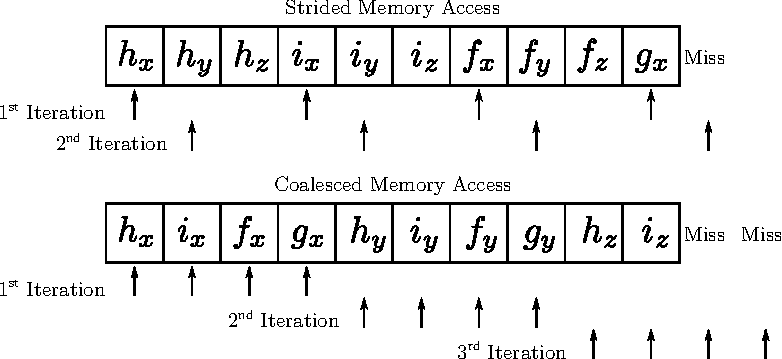
\includegraphics[width=\linewidth]{mem_access.pdf}
		\caption[Memory access pattern example.]{Arrows represent fetch requests by single threads in a GPU. Data should be arranged in such a way that all threads in a warp (collections of 32 threads) access contiguous memory locations to reduce time-consuming memory fetch operations. This is often unintuitive but extremely important, especially on scientific computing cards which are optimised for long computational times and low memory fetch frequency.}
		\label{f:mem_access}
	\end{figure}

	The difficulty in parallelisation varies tremendously from problem to problem. Problems where data is uncorrelated and independent---such as sampling well-behaved probability distributions---are almost trivially parallelisable. Problems where data is correlated or strongly dependent on its neighbours---such as Dislocation Dynamics---require a more careful approach \cite{parallel_algs}.
	
	The largest hurdle when implementing parallel algorithms is often the efficient use of data. In order to obtain good parallel performance, a lot of thought has to be placed on data access patterns, data read/write conflicts, and memory allocation and transfer \cite{nvidia}. For best performance, all this must be analysed on a case by case basis. If done incorrectly, the performance of a parallel application may be lower than the serial version. One must consider a wide range of parameters to successfully parallelise a problem. Among these are GPU architecture, problem size, computational and memory complexity, code branching, required arithmetic precision, and error tolerances \cite{nvidia, gpu_rev}.

	Efficient parallelisation of many problems requires ``coalesced memory access'' as shown in \cref{f:mem_access}, which means we have to be extremely careful when mapping CPU memory to global GPU (device) memory. The fact that threads work ``simultaneously''\footnote{Not quite but essentially simultaneously. See \cite{nvidia} for details.} means that in order to obtain good performance, data which is to be ``simultaneously'' loaded into each thread must be contiguous. This maximises cache memory use and therefore reduces slow memory fetch operations to global or shared memory.
	
	Special cases, such as having a parallel dislocation line segment to a surface as discussed in \cref{s:anal_forces}, must be treated carefully due to the way code branching works in GPUs. There are various ways of doing so:
	\begin{inparaenum}[\itshape 1\upshape)]
		\item if the special case is inexpensive, it can be treated within the same GPU function;
		\item if the special case is expensive and always known (certain boundary conditions in FEM), it can be placed in its own GPU function that treats it separately;
		\item if the special case is expesive and found at runtime it may be asynchronously treated by the CPU or buffered into its own GPU function to be executed at a later time.			
	\end{inparaenum}

	\begin{figure}[t]
		\centering
		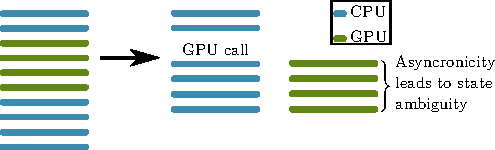
\includegraphics[width=\textwidth]{async.pdf}
		\caption[GPU and CPU asynchronous execution.]{GPU and CPU code run independent of each other. Leads to state ambiguities if both sides need to talk to each other \cite{nvidia}.}
		\label{f:async_gpu_cpu}
	\end{figure}
	One of the advantages of GPU-CPU independence is that both can work concurrently on the problem. If both systems have to talk to each other, then one must tread carefully, ensuring proper syncronisation and data mapping before moving (see \cref{f:async_gpu_cpu}).
		
	The reason why code branching is bad for GPU parallelisation is down to the fact that they work like software customisable vector machines. Where collections of threads all carry out the same operation on different pieces of data at the same time. This means that regardless of whether a condition is true or false, the code will execute. It is only data storage that depends on the condition. When working with CUDA, one must avoid code branching as much as possible, particularly rare but computationally expensive branches.

	Dislocation Dynamics (DD)---in particular 3D Discrete Dislocation Dynamics (3D DDD)---can greatly benefit from parallelisation, especially when coupling to Finite Element Methods (FEM). It is worth noting that there are potential issues arising from the very computationally expensive functions and special cases that often arise from analytical solutions in 3D DDD. There are also potential issues with data redundancy---which are non-limiting in the short term---that may eventually require a more data-efficient approach as the computational capabilities and data capabilities of GPUs converge. \Cref{s:para_ddd} expands on these issues in the context of DD.
    
	\section{Parallelisation on Graphics Processing Units}
	Efficient parallelisation requires coalesced memory access, which means we have to be extremely careful when mapping CPU memory to device memory. The fact that threads work ``simultaneously''\footnote{Not quite but essentially simultaneously.} means that in order to obtain good performance, data which is to be ``simultaneously'' loaded into each thread must be contiguous. This maximises cache memory use and therefore reduces slow memory fetch operations.
	%
	\subsection{Data Mapping}
		%
		\subsubsection{Elements: Host $ \mapsto $ Device}
			%
			\begin{algorithm}
				\caption{Elements in host $ \mapsto $ device.}
				\label{a:ehd}
				\begin{algorithmic}[1]
					\Function{element\_host\_device\_map}{\hvar{\vec{X}[N][3\times E]}}
						\State{$ i,\, j,\, k \gets 0 $}
						\State{$ \dvar{\vec{X}} \gets $ malloc($ 3\times E\times N $)}
						\For{$(n = 0;\, n < N;\, n++)$}
							\State{$ k \gets j $}
							\For{$ (c = 0;\, c < 3;\, c++) $}
								\State{$ i \gets c $}
								\For{$ (e = 0;\, e < E;\, e++) $}
									\State{$ \dvar{\vec{X}[k + e]} \gets \hvar{\vec{X}[n][i]} $}
									\State{$ i \gets i + 3 $}
								\EndFor
								\State{$ k \gets k + E \times N $}
							\EndFor
							\State{$ j \gets j + E $}
						\EndFor
						\State{\Return{\dvar{\vec{X}}}}
					\EndFunction
				\end{algorithmic}
			\end{algorithm}
		\subsubsection{Elements: Device $ \mapsto $ Thread}
			\begin{algorithm}
				\caption{Elements in device $ \mapsto $ thread.}
				\label{a:edt}
				\begin{algorithmic}[1]
						\GPUFunction[element\_device\_thread\_map]{\dvar{\vec{X}[3\times E\times N]}, \tvar{\vec{X}[N][3]}}
						\State{$ \rvar{idx},\, i \gets \rvar{threadIdx}.x + \rvar{blockIdx}.x\times \rvar{blockDim}.x $}
						\For{$ (c = 0;\, c < 3;\, c++) $}
							\For{$ (n = 0;\, n < N;\, n++) $}
								\State{$ \tvar{\vec{X}[n][c]} \gets \dvar{\vec{X}[i + n\times E]}$}
							\EndFor
							\State{$ i \gets i + E\times N $}
						\EndFor
						\State{\Return{\tvar{\vec{X}[n][c]}}}
					\EndGPUFunction
				\end{algorithmic}    	
			\end{algorithm}
		\subsubsection{Force: Thread $ \xmapsto{+} $ Device}
			\begin{algorithm}
				\caption{Force in thread $ \xmapsto{+} $ device.}
				\begin{algorithmic}[1]
						\GPUFunction[add\_force\_thread\_device]{\tvar{\vec{F_{n}}[N][3]}, \tvar{\vec{F_{e}}[3]}, \dvar{\vec{F_{n}}[3\times E\times N]},\newline{}\dvar{\vec{F_{e}}[3\times E]}, \rvar{idx}}
						\State{\Comment{Nodal force.}}
						\State{\Comment{Set output index to whatever parallelisation index is given to the function. In this case the same index we use for the main parallelisation.}}
						\State{$ i \gets \rvar{idx} $}
						\For{$ (n = 0;\, n < N;\, n++) $} \Comment{Loop over nodes.}
							\For{$ (c = 0;\, c < 3;\, c++) $} \Comment{Loop over coordinates.}
								\State{\Comment{Ensure nodal forces are correctly added and mapped from local thread memory to global device memory.}}
								\State{atomicAdd(\dvar{\vec{F_{n}}[i + c\times E\times N]}, \tvar{\vec{F_{n}}[n][c]})}
							\EndFor
							\State{\Comment{Displace output index to point at the first coordinate of the $ (n+1)\textsuperscript{th} $ node of the \rvar{idx}\textsuperscript{th} SE.}}
							\State{$ i \gets i + E $}
						\EndFor
						\State{\Comment{Total force.}}	
						\State{$ i \gets \rvar{idx} $} \Comment{Reset output index.}
						\For{$ (c = 0;\, c < 3;\, c++) $} \Comment{Loop over coordinates.}
							\State{atomicAdd(\dvar{\vec{F_{e}}[i]}, \tvar{\vec{F_{e}}[c]})}
							\State{\Comment{Advance the output index to point at the $ (i+1)\textsuperscript{th} $ coordinate of the $ \rvar{idx}\textsuperscript{th} $ SE.}}
							\State{$ i \gets i + E $}
						\EndFor
						\State{\Return{\dvar{\vec{F_{n}}}, \dvar{\vec{F_{e}}}}}
					\EndGPUFunction
				\end{algorithmic}
			\end{algorithm}
		\subsubsection{Force (Parallelise over Dislocations): Thread $ \xmapsto{+} $ Device}
			\begin{algorithm}
				\caption{Force (parallelise over dislocations) in thread $ \xmapsto{+} $ device.}
				\begin{algorithmic}[1]
					\GPUFunction[dln\_add\_force\_thread\_device]{\tvar{\vec{F_{n}}[N][3]}, \tvar{\vec{F_{e}}[3]},\newline{}\dvar{\vec{F_{n}}[3\times E\times N]}, \dvar{\vec{F_{e}}[3\times E]}, $ k $}
						\State{\Comment{Nodal force.}}
						\State{\Comment{Set output index to correspond to whatever SE we're on. By parallelising over dislocation lines, we must loop through SEs in the main code, this is the value of $ k $ we provide. Multiply by 3 and $ N $ because each SE has 3 coordinates and $ N $ nodes.}}
						\State{$ i \gets 3\times N\times k $}
						\State{$ j \gets 0 $} \Comment{Auxiliary index.}
						\For{$ (n = 0;\, n < N;\, n++) $} \Comment{Loop over nodes.}
							\For{$ (c = 0;\, c < 3;\, c++) $} \Comment{Loop over coordinates.}
								\State{\Comment{Ensure nodal forces are correctly added and mapped from local thread memory to global device memory.}}
								\State{atomicAdd(\dvar{\vec{F_{n}}[i + j + c]}, \tvar{\vec{F_{n}}[n][c]})}
							\EndFor
							\State{\Comment{Displace auxiliary index to point at the first coordinate of the $ (n+1)\textsuperscript{th} $ node of the $ k \textsuperscript{th}$ SE.}}
							\State{$ j \gets j + 3 $}
						\EndFor
						\State{\Comment{Total force.}}
						\State{\Comment{Set auxiliary index to point at the first coordinate of the $ k\textsuperscript{th} $ SE.}}
						\State{$ j \gets 3\times k $}
						\For{$ (c = 0;\, c < 3;\, c++) $} \Comment{Loop over coordinates.}
							\State{atomicAdd(\dvar{\vec{F_{e}}[j+c]}, \tvar{\vec{F_{e}}[c]})}
						\EndFor
						\State{\Return{\dvar{\vec{F_{n}}}, \dvar{\vec{F_{e}}}}}
					\EndGPUFunction
				\end{algorithmic}
			\end{algorithm}
		\subsubsection{Nodal Force: Device $ \mapsto $ Host}
			\begin{algorithm}
				\caption{Nodal force in device $ \mapsto $ host.}
				\begin{algorithmic}[1]
					\Function{fx\_device\_host\_map}{\dvar{\vec{F_{n}}[3\times E\times N]}, \hvar{\vec{F_{n}}[N][3\times E]}}
						\State{$ i,~j \gets 0 $} \Comment{Set input and output indices to zero.}
						\For{$ n = 0;\, n < N;\, n++ $} \Comment{Loop over nodes.}
							\State{$ j \gets 0 $} \Comment{Reset output index to point at the first element.}
							\For{$ e = 0;\, e < E;\, e++ $} \Comment{Loop over elements.}
								\For{$ c = 0;\, c < 3;\, c++ $} \Comment{Loop over coordinates.}
									\State{$ \hvar{\vec{F_{n}}[n][j + c]} = \dvar{\vec{F_{n}}[i + e + c\times E\times N]} $}
								\EndFor
								\State{\Comment{Advance output index to point at the first coordinate of the $ (e+1)\textsuperscript{th} $ element.}}
								\State{$ j \gets j + 3 $}
							\EndFor
							\State{\Comment{Advance input index to point at the first coordinate of the $ (n+1)\textsuperscript{th} $ node of the first element.}}
							\State{$ i \gets i + E $}
						\EndFor
						\State{\Return{\hvar{\vec{F_{n}}}}}
					\EndFunction
				\end{algorithmic}
			\end{algorithm}
		\subsubsection{Total Force: Device $ \mapsto $ Host}
			\begin{algorithm}
				\caption{Total force in device $ \mapsto $ host.}
				\begin{algorithmic}[1]
					\Function{ftot\_device\_host\_map}{\dvar{\vec{F_{e}}[3\times E]}, \hvar{\vec{F_{e}}[3\times E]}}
						\State{$ i \gets 0 $} \Comment{Set output index to zero.}
						\For{$ e = 0;\, e < E;\, e++ $} \Comment{Loop over elements.}
							\For{$ c = 0;\, c < 3;\, c++ $} \Comment{Loop over coordinates.}
								\State{$ \hvar{\vec{F_{e}}[i + c]} = \dvar{\vec{F_{e}}[e + c\times E]} $}
							\EndFor
							\State{\Comment{Advance the output index to point at the first coordinate of the $ (e+1)\textsuperscript{th} $ surface element.}}
							\State{$ i \gets i + 3 $}
						\EndFor
						\State{\Return{\hvar{\vec{F_{e}}}}}
					\EndFunction
				\end{algorithmic}
			\end{algorithm}
	\begin{subequations}\label{e:fcne}
		\begin{align}
			\vec{X}_{en}			&\coloneqq	\left[x_{en},\, y_{en},\, z_{en}\right]\\
			\vec{X}_{(1\to E)n}		&\mapsto 	\vec{X}_{n} \nn
			\vec{X}_{n}				&\coloneqq	\left[x_{1n},\, y_{1n},\, z_{1n},\ldots,x_{En},\, y_{En},\, z_{En}\right]\label{se:xn_arr}\\
			\vec{X}_{1\to N}		&\mapsto	\vec{X}^{\textrm{SE}}\nn
			\vec{X}^{\textrm{SE}}	&\coloneqq 
			\begin{aligned}
				&\left[x_{11},\, \ldots,\, x_{E1},\, x_{12},\, \ldots,\, x_{E2},\, \ldots,\, x_{1N},\, \ldots,\, x_{EN}, \right.\\
				&\left.\,y_{11},\, \ldots,\, y_{E1},\, y_{12},\, \ldots,\, y_{E2},\, \ldots,\, y_{1N},\, \ldots,\, y_{EN}, \right.\\
				&\left.\,z_{11},\, \ldots,\, z_{E1},\, z_{12},\, \ldots,\, z_{E2},\, \ldots,\, z_{1N},\, \ldots,\, z_{EN}  \right]
			\end{aligned}
		\end{align}
	\end{subequations}
	where $ e $ is the SE label, $ n $ the node label, $ E $ the number of SEs in the scope. $ N $ the number of nodes in a SE.
	
	Data-mapping according to \cref{a:fcne} and relabelling the nodes so they go from $ 0 \to N-1 $, the data from \cref{f:lrse_map} would be arranged in device memory like \cref{e:fcne_eg},
	\begin{align}\label{e:fcne_eg}
		\vec{X}^{\textrm{SE}} &= \begin{aligned}
			\left[\underbrace{h_{x},\, i_{x},\, f_{x},\, g_{x}}_{\mathbf{x_{0}}},\, 
			\underbrace{a_{x},\, b_{x},\, i_{x},\, h_{x}}_{\mathbf{x_{1}}},\, 
			\right.&\underbrace{i_{x},\, d_{x},\, e_{x},\, f_{x}}_{\mathbf{x_{2}}},\, 
			\underbrace{b_{x},\, c_{x},\, d_{x},\, i_{x}}_{\mathbf{x_{3}}},\\
			\ldots~y&\textrm{-coord}~\ldots,\\
			\ldots~z&\textrm{-coord}~\ldots]
		\end{aligned}
	\end{align}
	%
	
	In the GPU, each thread will cater to one SE at a time. This means that each thread will have to extract the relevant data from the 1D array with length $ 3\times E\times N $ into four 1D arrays of length $ 3 $. The purpose of CNE mapping is to provide the warp with coalesced memory access. This is achieved via \cref{a:bcne}.
	
	
	Since \cref{a:bcne} is performed in a CUDA GPU, threads in a single block execute sequentially from,
	\begin{align}
		\rvar{threadIdx}.x &= 0 \to \rvar{threadIdx}.x = \rvar{blockDim}.x - 1\,,
	\end{align}
	while threads in different blocks execute in parallel. coalesced memory access is ensured by having each block load a cache line whose entries are contiguously accessed by the threads in the block. Using the same notation as \cref{a:fcne}, full cache line utilisation (optimal cache use) is achieved if cache lines can accomodate $ l $ entries given by \cref{e:opt_cache_len_bcne},
	\begin{align}
		\label{e:opt_cache_len_bcne}
		l =
		\begin{cases}
			a \times N \times E &,\, a > 0 \in \mathbb{N}\\
			&\textrm{or}\\
			\dfrac{1}{2^{a}} \times N \times E &,\, a \geq 0 \in \mathbb{N},\, N \times E \equiv 0\; (\bmod\; 2^{a})\,.
		\end{cases}
	\end{align}
	\subsubsection{Node Coordinate Element Map}
	%
	The node-coordinate-element (NCE) data mapping in \cref{e:fnce} is carried out by \cref{a:fnce}, each thread looks after a given SE.
	\begin{algorithm}
		\caption{NCE data mapping.}
		\label{a:fnce}
		\begin{algorithmic}
			\ForAll{n nodes $ \in $ surface element}
			\ForAll{c coordinates $ \in [x,\, y,\, z] $}
			\ForAll{e surface elements $ \in $ surface mesh section}
			\State list.append(data of the $ n\textsuperscript{th}$ node with $ c\textsuperscript{th} $ coordinate of the $ e\textsuperscript{th} $ SE)
			\EndFor
			\EndFor
			\EndFor
		\end{algorithmic}
	\end{algorithm}
	\begin{subequations}\label{e:fnce}
		\begin{align}
			\vec{X}_{en}			&\coloneqq \left[x_{en},\, y_{en},\, z_{en}\right]\\
			\vec{X}_{(1\to E)n}		&\mapsto \vec{X}_{n} \nn
			\vec{X}_{n}				&\coloneqq \left[x_{1n},\ldots,\, x_{En},\, y_{1n},\ldots,\, y_{En},\, z_{1n},\ldots,\, z_{En}\right]\\
			\vec{X}_{1\to N}		&\mapsto \vec{X}^{\textrm{SE}}\nn
			\vec{X}^{\textrm{SE}}	&\coloneqq 
			\begin{aligned}
				\left[x_{11},\ldots,\, x_{E1},\, y_{11},\right.&\ldots,\, y_{E1},\, z_{11},\ldots,\, z_{E1}\\
				,&\ldots,\\
				x_{1M},\ldots,\, x_{EN},\, y_{1N},&\left.\ldots,\, y_{EN},\, z_{1N},\ldots,\, z_{EN}\right]
			\end{aligned}
		\end{align}
	\end{subequations}
	where $ e $ is the surface \textbf{e}lement, $ n $ the \textbf{n}ode, $ E $ the total number of SEs in scope, $ N $ the total number of nodes in each SE.
	
	Data-mapping according to \cref{a:fnce} and relabelling the nodes so they go from $ 0 \to N-1 $, the data from \cref{f:lrse_map} would be arranged in device memory like \cref{e:fnce_eg},
	\begin{align}\label{e:fnce_eg}
		\vec{X}^{\textrm{SE}} &= \begin{aligned}
			&\left[\underbrace{h_{x},\, i_{x},\, f_{x},\, g_{x},\, 
				h_{y},\, i_{y},\, f_{y},\, g_{y},\, 
				h_{z},\, i_{z},\, f_{z},\, g_{z}}_{\mathbf{x_{0}}}\right.,\\
			&~\ldots~\mathbf{x_{1}},\, xyz\textrm{-coords}~\ldots,\\
			&~\ldots~\mathbf{x_{2}},\, xyz\textrm{-coords}~\ldots,\\
			&~\ldots~\mathbf{x_{3}},\, xyz\textrm{-coords}~\ldots]
		\end{aligned}
	\end{align}
	%
	\subsubsection{Resolving Data Write Conflicts}
	Data write conflicts can be a problem in parallel applications where global data is changed by multiple threads within the same clock tick. This can be avoided with atomic operations.
	%
	\subsection[Parallel Dislocation Line Segments to Surface Elements]{Resolving Parallel Dislocation Line Segments to Surface Elements}
	%
	Dealing with the special case when the dislocation line segment $ \vec{t} $ is parallel to the SE is relatively trivial when in a serial program. By the mean value theorem, we can slightly perturb $ \vec{t} $ by rotating it by a small angle around the midpoint of $ \vec{t} $ with respect to the axis of rotation defined by $ \vec{t} \times \vec{n} $. In contrast to serial code, program branches can have a serious effect on parallel performance due to warp divergence. Due to the complexity of the force calculation and relative rarity of the edge case, there is no branching behaviour in the parallel code until \emph{after} the calculation is performed. Where \cref{a:plse_p} is performed.
	\begin{algorithm}
		\caption{Resolving cases when $ \vec{t} \parallel \vec{n} $ on GPUs.}
		\label{a:plse_p}
		\begin{algorithmic}
			\ForAll{surface elements \emph{and} line segments}
			\State $ \ldots $
			\If{$ \vec{t}_{\textrm{thread}} \parallel \vec{n}_{\textrm{thread}} $}
			\State $ \vec{x}_{\textrm{buffer}} \gets \vec{x}_{\textrm{thread}} $
			\State $ \vec{t}_{\textrm{buffer}} \gets \vec{t}_{\textrm{thread}} $
			\Else
			\State $ \vec{F}_{\textrm{total}} += \vec{F}_{\textrm{thread}} $
			\EndIf
			\EndFor
			\State return to serial code
			\If{$ \vec{x}_{\textrm{buffer}} \neq $ empty}
			\ForAll{surface elements \emph{and} line segments}
			\State perform calculation for $ \vec{t} \parallel \vec{n} $
			\EndFor
			\EndIf
		\end{algorithmic}
	\end{algorithm}

\section{Theory}\label{s:theory}

\section{Methodology}\label{s:method}
        
\section{Results}

\section{Acknowledgements}

We would like to thank Prof. Sylvain Queyreau and Lawrence Livermore National Laboratory for their invaluable input. This work was supported by the Consejo Nacional de Ciencia y Tecnologia, Fondo Sectorial CONACYT-Secretaria de Energia-Sustentabilidad Energetica Cuarto Periodo [291129]. This work was supported by the Engineering and Physical Sciences Research Council Centre for Doctoral Training in the Science and Technology of Fusion Energy EP/L01663X/1 and Fellowship grant EP/N007239/1.
  %% References
  %%
  %% Following citation commands can be used in the body text:
  %% Usage of \cite is as follows:
  %%   \cite{key}          ==>>  [#]
  %%   \cite[chap. 2]{key} ==>>  [#, chap. 2]
  %%   \citet{key}         ==>>  Author [#]

  %% References with bibTeX database:
  \newcommand{\newblock}{}
  \bibliographystyle{unsrtnat}
  \bibliography{references.bib}

  %% Authors are advised to submit their bibtex database files. They are
  %% requested to list a bibtex style file in the manuscript if they do
  %% not want to use model1-num-names.bst.

  %% References without bibTeX database:

  % \begin{thebibliography}{00}

  %% \bibitem must have the following form:
  %%   \bibitem{key}...
  %%

  % \bibitem{}

  % \end{thebibliography}
\end{document}

%%
%% End of file `elsarticle-template-1-num.tex'.